\documentclass{ctexart}
\usepackage[utf8]{inputenc}
\usepackage{graphicx}
\usepackage{amsmath}
\usepackage{amssymb}
\usepackage{enumitem}

\title{数值分析 - 第四次实验报告}
\author{强基数学2001班 樊睿}
\date{2022.11.17}

\begin{document}

\maketitle

\section{第一题}

\subsection{题目描述}

直接计算以下三个函数 $f,g,h$ 在区间 $[0,99,1.01]$ 上 $101$ 个等距点上的函数值并作图。注意这三个函数在理论上是完全相同的。观察结果并解释原因。

\subsection{代码实现}

计算数据代码:

\begin{verbatim}
#include<bits/stdc++.h>
#include"../HW1/function.h"
using namespace std;

class F : public Function<double> {
public:
    virtual double operator()(const double& x) const{
    return x*x*x*x*x*x*x*x-8*x*x*x*x*x*x*x+28*x*x*x*x*x*x-56*x*x*x*x*x+70*x*x*x*x-56*x*x*x+28*x*x-8*x+1;
    }
}f;

class G : public Function<double> {
public:
    virtual double operator()(const double& x) const{
        return (((((((x-8)*x+28)*x-56)*x+70)*x-56)*x+28)*x-8)*x+1;
    }
}g;

class H : public Function<double> {
public:
    virtual double operator()(const double& x) const{
    return (x-1)*(x-1)*(x-1)*(x-1)*(x-1)*(x-1)*(x-1)*(x-1);
    }
}h;

int main(){
    ofstream out("A.csv");
    out<<"x,f,g,h\n";
    for(int i=0;i<=100;++i){
    double x=0.99+i*0.0002;
    out<<x<<','<<f(x)<<','<<g(x)<<','<<h(x)<<'\n';
    }
}
\end{verbatim}

作图代码:

\begin{verbatim}
import matplotlib.pyplot as plt
import numpy as np
import pandas as pd

file = pd.read_csv("A.csv")

data = pd.DataFrame(file)
plt.plot(data['x'], data['f'])
plt.plot(data['x'], data['g'])
plt.plot(data['x'], data['h'])
plt.show()
\end{verbatim}

\subsection{运行结果}
三个函数各自的101个点值已存入\verb|A.csv|中。图像如下。蓝色、橙色和绿色的曲线分别为 $f,g,h$ 的函数图像。

\begin{figure}[h]
    \begin{minipage}{4cm}
	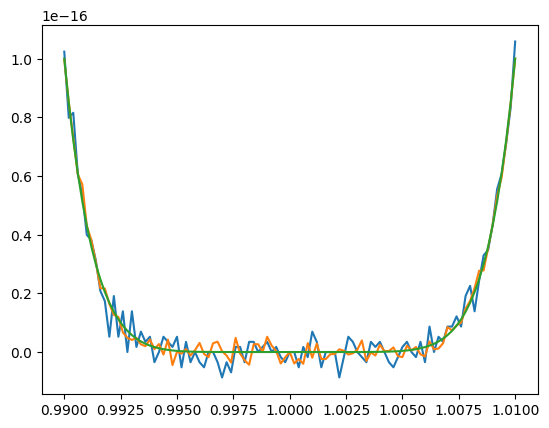
\includegraphics[width = 12cm, height = 8cm]{A.png}
	\label{fig1}
	\end{minipage}
\end{figure}

\subsection{结果分析}

$f,g$ 的计算结果在 $x\rightarrow 1$ 时很不精确,$h$ 的计算结果在 $x\rightarrow 1$ 时较精确。

三个函数在理论上相同,因此条件数也相同,均为 $|\frac {8x}{x-1}|$。故 $x$ 在 $1$ 附近时条件数均趋于无穷。无论什么计算方法在 $x$ 非常接近 $1$ 时都是不精确的。

但 $f$ 和 $g$ 在最后一步时,其实要计算的是 $(f(x)-1)+1$,由于 $f(x)$ 非常接近 $1$,在 $10^{-16}$ 到 $10^{-30}$ 之间,已经接近甚至小于 $\varepsilon_u=2.2\times 10^{-16}$。因此即使不计前面计算产生的误差,仅这一步就会带来极其严重的巨量消失,所有的有效位数全都被舍入了。因此 $f,g$ 的计算结果可以认为是毫无意义的。而 $h$ 只有在计算 $x-1$ 时会损失一部分精度,因为 $x-1$ 的数量级为 $10^{-4}$ 以上,远高于 $\varepsilon_u$,所以精度损失几乎可忽略不计。

所以对于本例,$h$ 的精度比 $f,g$ 好得多。但从理论上可以分析,当 $x-1$ 的数量级进一步降低,降到 $\varepsilon_u$ 附近时,$h$ 的精度也会严重下降。

\section{第二题}

\subsection{题目描述}
考虑 $\beta=2,p=3,L=-1,U=1$ 的正则浮点系统 $\mathbb{F}$。
\begin{itemize}
\item 计算 $UFL(\mathbb{F})$ 和 $OFL(\mathbb{F})$。
\item 列举 $\mathbb{F}$ 中所有的浮点数,并验证讲义中关于 $\#\mathbb{F}$ 的推论。
\item 在数轴上画出 $\mathbb{F}$。
\item 列举 $\mathbb{F}$ 中所有的非正则浮点数。
\item 在数轴上画出扩展的 $\mathbb{F}$。
\end{itemize}

\subsection{代码实现}
\begin{verbatim}
#include<bits/stdc++.h>
using namespace std;

int main(){
    double UFL = 1.0 / 2;
    double OFL = 2 * (2 - 1.0 / 4);
    cout << "UFL = " << UFL << endl;
    cout << "OFL = " << OFL << endl;
    vector <double> num;
    vector <double> subnum;
    num.push_back(0);
    double base = 1.0 / 2;
    for (int e = -1; e <= 1; ++ e) {
        double M;
        for (int i = 0; i < 2; ++ i)
            for (int j = 0; j < 2; ++ j) {
                for (int k = 0; k < 2; ++ k) {
                    M = i + j / 2.0 + k / 4.0;
                    if (i > 0) {
                        num.push_back(M * base);
                        num.push_back(-M * base);
                    }
                    else {
                        if (e == -1) {
                            subnum.push_back(M * base);
                            subnum.push_back(-M * base);
                        }
                    }
                }
            }
        base *= 2;
    }
    sort(num.begin(), num.end());
    cout << "numbers(" << num.size() << "):\n";
    for (double x : num) cout << x << ",\n"[x == num.back()];
    sort(subnum.begin(), subnum.end());
    cout << "subnumbers(" << subnum.size() << "):\n";
    for (double x : subnum) cout << x << ",\n"[x == subnum.back()];
}
\end{verbatim}

\subsection{问题解答}

$UFL(\mathbb{F})=\beta^L=2^{-1}=0.5$

$OFL(\mathbb{F})=\beta^U(\beta-beta^{1-p})=2^1(2-2^{-2})=3.5$

正则浮点数(25个):-3.5,-3,-2.5,-2,-1.75,-1.5,-1.25,-1,-0.875,-0.75,-0.625,-0.5,0,0.5,0.625,0.75,0.875,1,1.25,1.5,1.75,2,2.5,3,3.5

非正则浮点数(8个):-0.375 -0.25 -0.125 0 -0 0.125 0.25 0.375

验证结论:$25=2^3(1-(-1)+1)+1$。

在数轴上画出:

\begin{figure}[h]
    \begin{minipage}{4cm}
	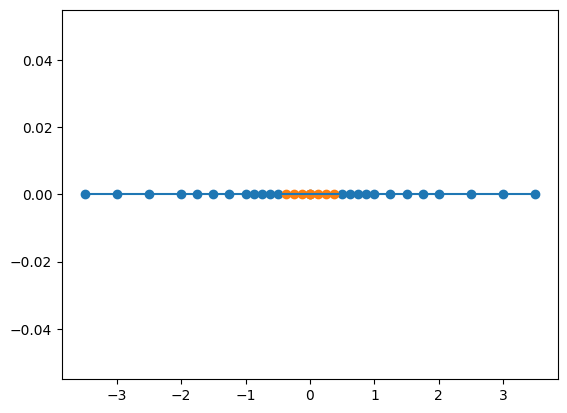
\includegraphics[width = 12cm, height = 8cm]{B.png}
	\label{fig1}
	\end{minipage}
\end{figure}

\end{document}
